\chapter{Epidemiología del cáncer}

La Epidemiología se ha definido tradicionalmente como el estudio de la distribución y de los determinantes de la enfermedad en los seres humanos [1]. En un sentido más amplio, sin limitarse únicamente a la enfermedad, la epidemiología se define como el estudio de la aparición y distribución de los estados o acontecimientos relacionados con la salud en poblaciones específicas, incluyendo el estudio de los determinantes de estos estados, y la aplicación de este conocimiento al control de los problemas de la salud [2, 3].\\

[1] MacMahon B, Pugh TF. Principios y métodos de Epidemiología. Segunda edición. México: La Prensa Médica Mexicana, 1983.
[2] Last JM. Diccionario de Epidemiología. Barcelona: Salvat, 1989.
[3] Porta M (editor). A Dictionary of Epidemiology (5th edition). New York: Oxford University Press; 2008.


\section{Indicadores epidemiológicos}

Para medir en la población el impacto del cáncer se utilizan principalmente cuatro indicadores:

\begin{itemize}
	\item \textbf{Incidencia} (casos nuevos). Mide el riesgo de presentar cáncer.
	\item \textbf{Mortalidad} (defunciones). Mide el riesgo de morir por cáncer.
	\item \textbf{Supervivencia} (porcentaje de casos vivos). Mide la historia natural del cáncer y efectividad del tratamiento.
	\item \textbf{Prevalencia} (casos nuevos y antiguos, vivos). Mide la carga asistencial de la enfermedad.
\end{itemize}

\textcolor{red}{Añadir tendencias}\\

% ---------------------------------

\textbf{Referencias:}

GLOBOCAN - \cite{Bray2018, GCO}

ECIS - \cite{ECIS, ECIS2}

REDECAN - \cite{REDECAN2020}

Población INE - \cite{INEpob}

Defunciones Ministerio - \cite{MSCBS}.

\section{Incidencia de cáncer}

Para medir de manera precisa la incidencia de cáncer en una población es necesaria la existencia de un Registro de Cáncer Poblacional. Estas entidades se dedican a registrar exhaustivamente todos los casos de cáncer diagnosticados en un área geográfica, y sus datos son muy útiles para todo tipo de estudios epidemiológicos. Algunos de estos Registros cubren la población de todo un país (por ejemplo, Canadá) mientras que otros cubren regiones concretas (por ejemplo, la provincia de Granada). Desgraciadamente, muchas áreas geográficas no están cubiertas por un Registro de Cáncer Poblacional. Es el caso de España, en el que sólo el 27\% de la población está cubierta por un Registro de Cáncer Poblacional \cite{Redondo-Sanchez2019}. Para conocer de manera estimada la incidencia de cáncer en territorios sin Registro de Cáncer Poblacional o proyectar la incidencia a años posteriores se utilizan diversos métodos matemáticos y estadísticos \cite{Bray2018, GCO, ECIS, ECIS2, REDECAN2020, Redondo-Sanchez2019}.\\

Con respecto a las medidas usadas para reportar la incidencia, la más sencilla y fácil de interpretar es el número nuevo de casos de cáncer, enmarcado siempre en un periodo concreto de tiempo y un área geográfica. A partir del número de casos se puede calcular la tasa bruta (TB), un indicador que tiene en cuenta el tamaño de la población \cite{IARC1995}.\\

$$\text{TB}  = \dfrac{\text{Número de casos nuevos}}{\text{Personas-año a riesgo}} \cdot 100.000 $$\\

Para permitir comparaciones entre distintas poblaciones, o la misma población en momentos distintos, es necesario tener en cuenta la estructura de edad de la población. Para responder a esta motivación se define la tasa estandarizada por edad (ASR por sus siglas en inglés, \textit{Age-Standardised Rate}) como aquella tasa que habría en la población de estudio si tuviese exactamente la misma estructura de edad que una población estándar predefinida \cite{IARC1995}. La definición de la tasa estandarizada por edad para 18 grupos de edad quinquenales (0-4 años, 5-9 años, $\dots$, 80-84 años, 85 años y más) es la siguiente:

$$\text{ASR} = \sum_{i = 1}^{18} \omega_i \dfrac{N_i}{P_i} $$
donde $N_i$ y $P_i$ son respectivamente el número de casos incidentes y la población en el $i$-ésimo grupo de edad, y $\omega_i$ es el peso que toma la población de referencia en el grupo $i$-ésimo, con $\sum_{i = 1}^{18}\omega_i = 100.000$. Los valores de ${\omega_i}$ están predefinidos en base a poblaciones estándar, siendo las más utilizadas en nuestro contexto las siguientes:

\begin{itemize}
	
	\item Población mundial. Propuesta por primera vez en 1960 \cite{SegiM.1960} y modificada más tarde en 1966 \cite{Doll1966}, permite realizar comparaciones a nivel mundial.
		
	\item Antigua población estándar europea. Propuesta en 1976 \cite{Waterhouse1976} basándose en la estructura de edad de varias poblaciones escandinavas, permite comparaciones entre zonas europeas.
	
	\item Nueva población estándar europea. En el año 2013, la Oficina Europea de Estadística (EUROSTAT) realiza una revisión de la población estándar europea con el objetivo de que la población refleje fielmente el envejecimiento existente en la población europea \cite{EUROSTAT2013}. Debido a su novedad, el uso de esta población aún no está ampliamente extendido en los organismos internacionales \cite{ECIS2} y en ocasiones se reportan las dos tasas estandarizadas por las poblaciones estándar antigua y nueva \cite{ECIS}.
	

\end{itemize}

En la Tabla 1 se muestran los pesos para cada una de las poblaciones de referencia mencionadas anteriormente.\\

\newpage
\textbf{Tabla 1}. Pesos de las poblaciones estándar para el cálculo de tasas estandarizadas por edad.
\begin{table}[H]
	\begin{tabular}{|c|c|c|c|}
		\hline
		
		Grupo de edad  &  \begin{tabular}[c]{@{}c@{}}Población estándar\\ mundial\end{tabular}  &  \begin{tabular}[c]{@{}c@{}}Población estándar\\ europea 1976\end{tabular}  &  \begin{tabular}[c]{@{}c@{}}Población estándar\\ europea 2013\end{tabular}\\\hline
		
		0-4 años  &  12.000  &  8.000  &  5.000\\
		5-9 años  &  10.000  &  7.000  &  5.500\\
		10-14 años  &  9.000  &  7.000  &  5.500\\
		15-19 años  &  9.000  &  7.000  &  5.500\\
		20-24 años  &  8.000  &  7.000  &  6.000\\
		25-29 años  &  8.000  &  7.000  &  6.000\\
		30-34 años  &  6.000  &  7.000  &  6.500\\
		35-39 años  &  6.000  &  7.000  &  7.000\\
		40-44 años  &  6.000  &  7.000  &  7.000\\
		45-49 años  &  6.000  &  7.000  &  7.000\\
		50-54 años  &  5.000  &  7.000  &  7.000\\
		55-59 años  &  4.000  &  6.000  &  6.500\\
		60-64 años  &  4.000  &  5.000  &  6.000\\
		65-69 años  &  3.000  &  4.000  &  5.500\\
		70-74 años  &  2.000  &  3.000  &  5.000\\
		75-79 años  &  1.000  &  2.000  &  4.000\\
		80-84 años  &  500  &  1.000  &  2.500\\
		$\geq$85 años  &  500  &  1.000  &  2.500\\\hline
		
	\end{tabular}
\end{table}

Para utilizar notación internacional, la tasa estandarizada por la población mundial se notará ASR-W (\textit{Age-Standardised Rate, World standard population}), la tasa estandarizada por la población europea de 1976 se notará ASR-oE (\textit{old European standard population}) y la de 2013 se notará ASR-nE (\textit{new European standard population}).\\

\subsection{Incidencia del total del cáncer excepto piel no melanoma}

\textcolor{red}{Poca importancia de piel no melanoma}\\

\newpage
\textbf{\textcolor{red}{Figura XX}}. Diagrama de Marimekko/mosaico con la incidencia estimada de cáncer en el mundo para el año 2018.
\begin{center}
	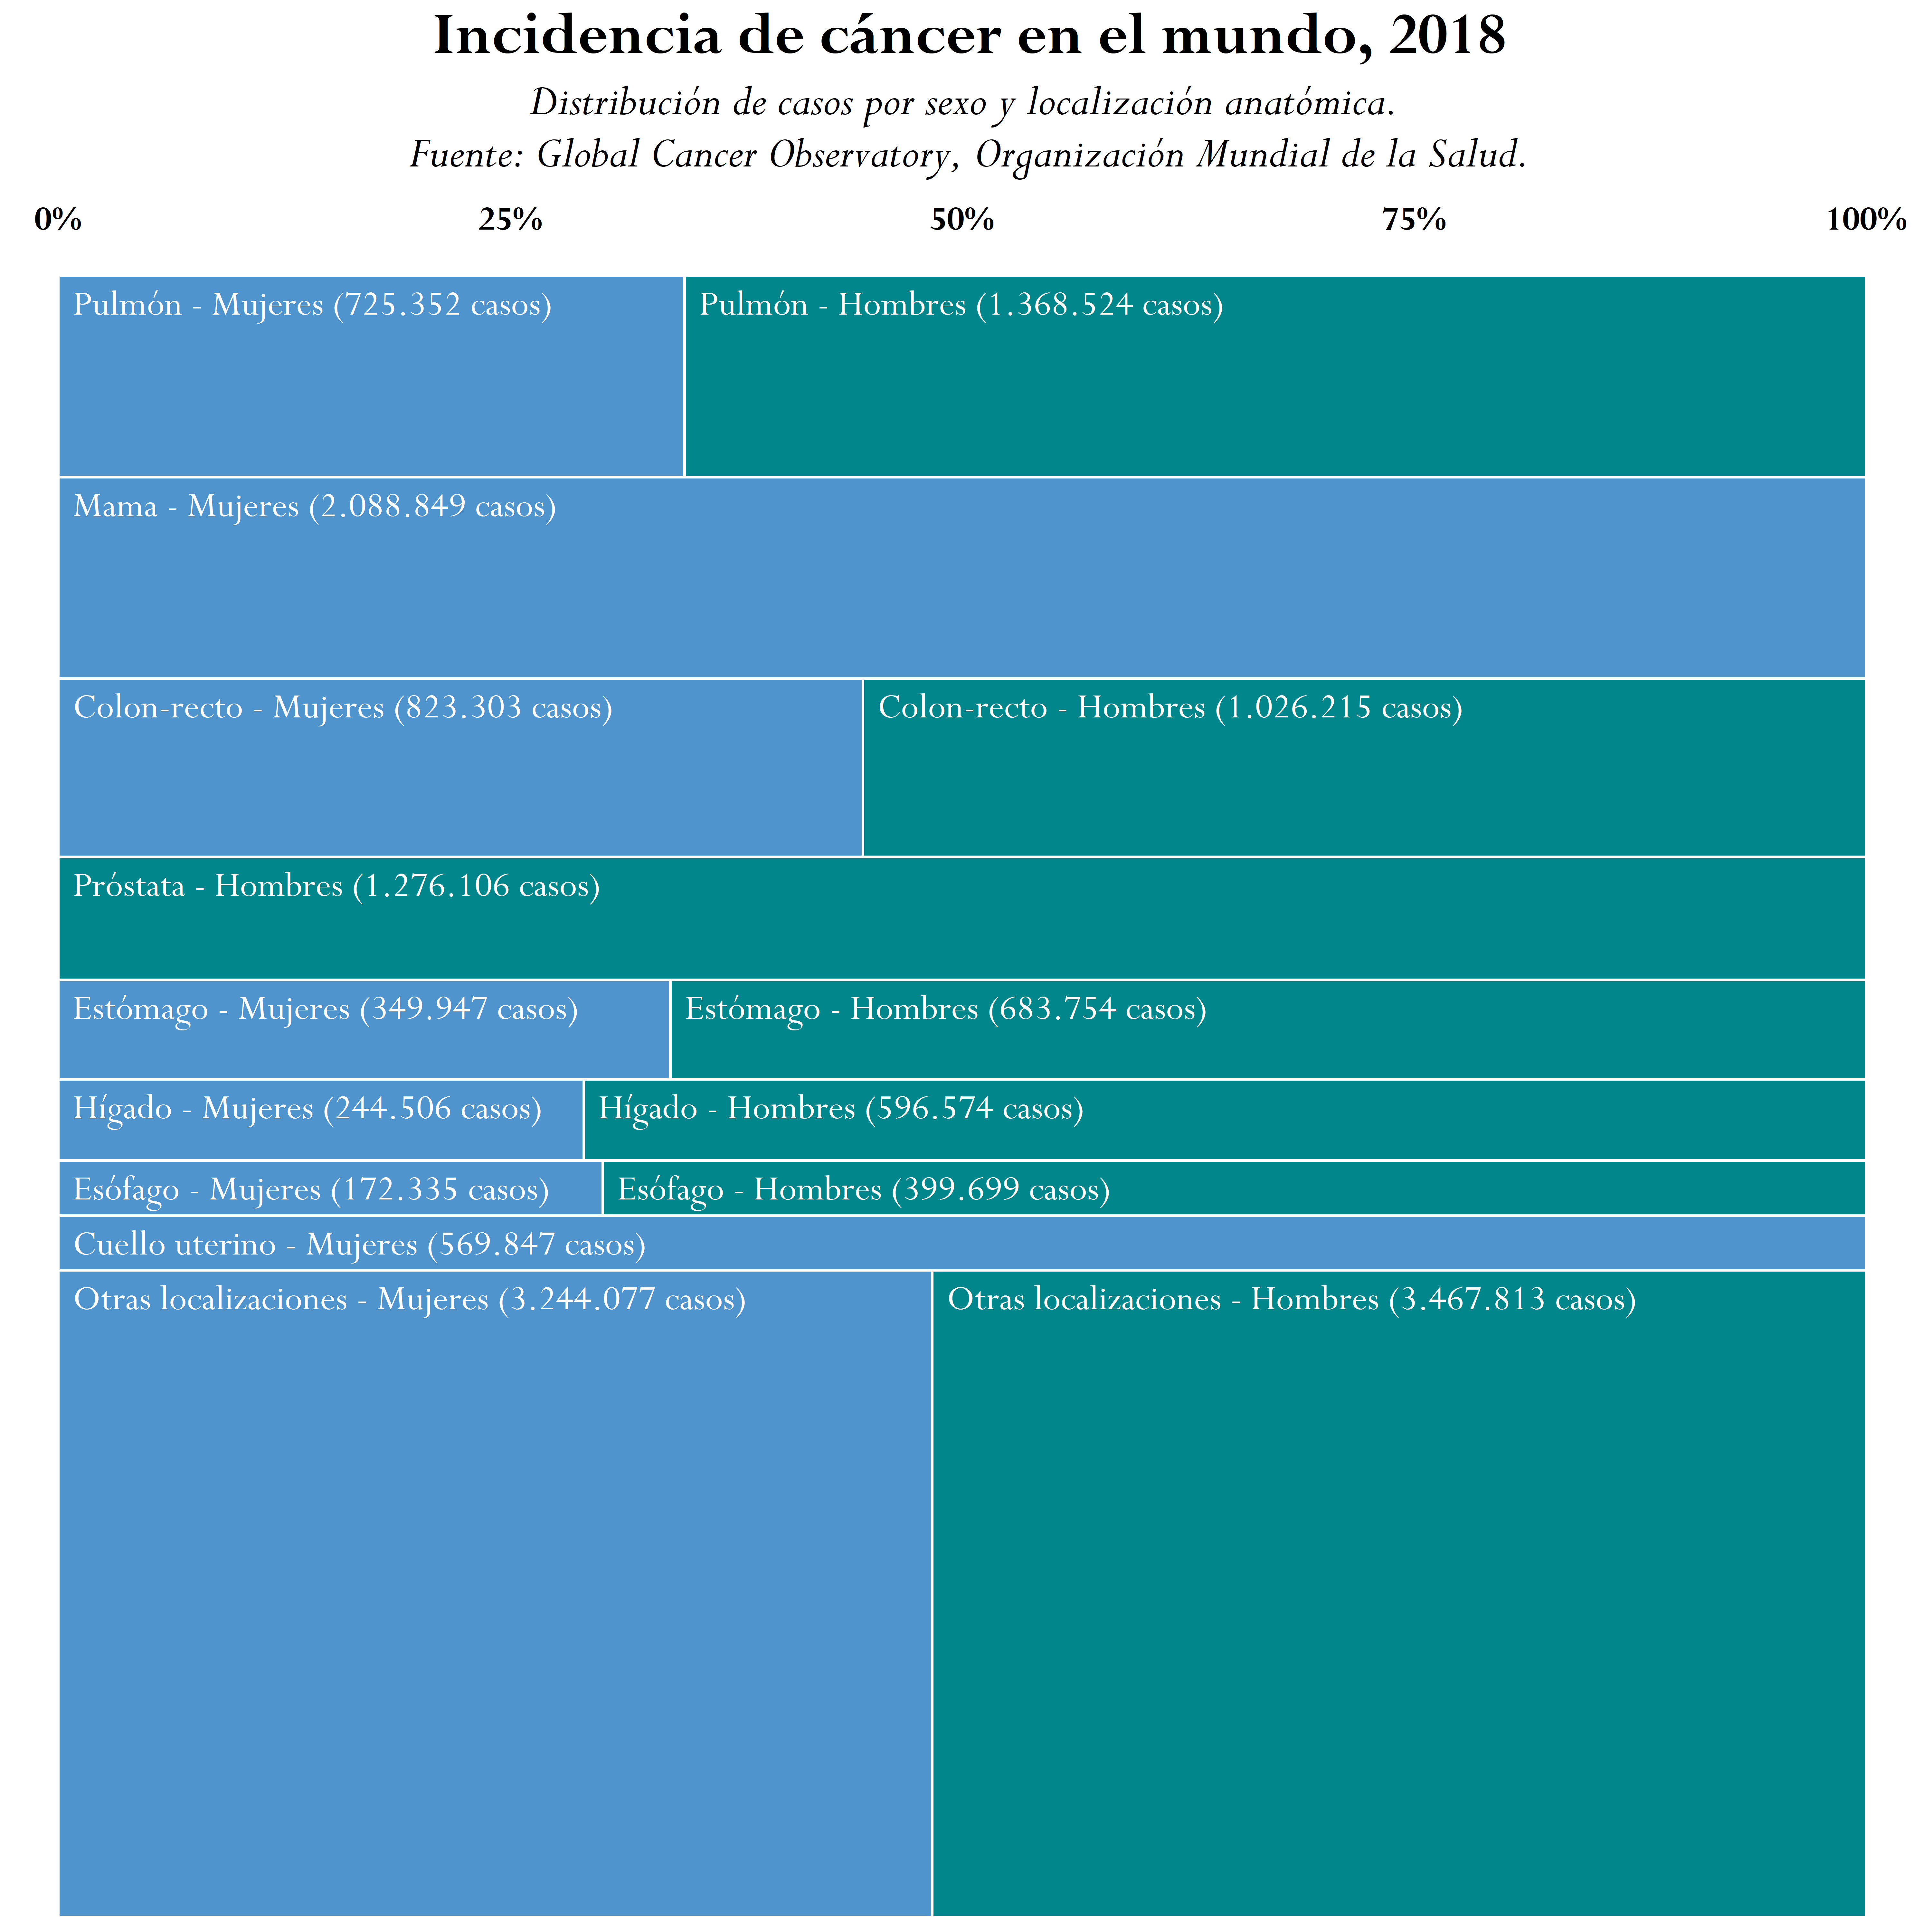
\includegraphics[width=1\textwidth]{figuras/marimekko_gco.png} \\
\end{center}


\subsection{Incidencia de cáncer de hígado}

texto

\subsection{Incidencia de cáncer de colon-recto}

texto

\section{Mortalidad por cáncer}

\textcolor{red}{Cómo se obtiene la mortalidad. Importancia de certif de defunción. También estimaciones y proyecciones.}

\subsection{Mortalidad del total del cáncer excepto piel no melanoma}

texto

\subsection{Mortalidad de cáncer de hígado}

texto

\subsection{Mortalidad de cáncer de colon-recto}

texto

\section{Supervivencia de cáncer} 

\textcolor{red}{Supervivencia se calcula principalmente a partir de inc, mort y tablas de vida población general}

\subsection{Supervivencia del total del cáncer excepto piel no melanoma}

texto

\subsection{Supervivencia de cáncer de hígado}

texto

\subsection{Supervivencia de cáncer de colon-recto}

texto

\section{Prevalencia de cáncer}

texto

\subsection{Prevalencia del total del cáncer excepto piel no melanoma}

texto

\subsection{Prevalencia de cáncer de hígado}

texto

\subsection{Prevalencia de cáncer de colon-recto}

texto






